\documentclass[10pt,twocolumn,letterpaper]{article}

\usepackage{cvpr}
\usepackage{times}
\usepackage{epsfig}
\usepackage[utf8]{inputenc}
\usepackage{romannum}
\usepackage{graphicx}
\usepackage{caption,subcaption}
\usepackage{listings}
\usepackage{color}
\usepackage{url}
\usepackage{amsmath}
\usepackage{nccmath}
\usepackage{mathtools}
% \usepackage{hyperref}
\usepackage{verbatim}
\usepackage{multirow}
\usepackage{bm}
\usepackage{amsmath}
\usepackage{amssymb}

% Include other packages here, before hyperref.

% If you comment hyperref and then uncomment it, you should delete
% egpaper.aux before re-running latex.  (Or just hit 'q' on the first latex
% run, let it finish, and you should be clear).
\usepackage[breaklinks=true,bookmarks=false]{hyperref}

\cvprfinalcopy % *** Uncomment this line for the final submission

\def\cvprPaperID{****} % *** Enter the CVPR Paper ID here
\def\httilde{\mbox{\tt\raisebox{-.5ex}{\symbol{126}}}}

% Pages are numbered in submission mode, and unnumbered in camera-ready
%\ifcvprfinal\pagestyle{empty}\fi
\setcounter{page}{4321}
\begin{document}

%%%%%%%%% TITLE
\title{Revisiting paper ``What makes an image memorable''}

\author{Darley Barreto, Edgar Tanaka, Tiago Barros\\
University of Campinas\\
{\tt\small \{darleybarreto, edgartanaka, tiago.ec09\}@gmail.com}
% For a paper whose authors are all at the same institution,
% omit the following lines up until the closing ``}''.
% Additional authors and addresses can be added with ``\and'',
% just like the second author.
% To save space, use either the email address or home page, not both
% \and
% Edgar Tanaka\\
% Institution2\\
% First line of institution2 address\\
% {\tt\small secondauthor@i2.org}
}

\maketitle
%\thispagestyle{empty}

%%%%%%%%% ABSTRACT
\begin{abstract}
    We know that some images stick to our memories more than others. Previous studies have identified that images carry the attribute of memorability, a value of whether an image will be later remembered or forgotten. Despite the potential overflow of visual information, humans are extremely good at remembering thousands of pictures along with some of their visual details. This work is based on the one performed by Isola et al. called ``What makes an image memorable?''. Their research has shown that memorability is a stable property of an image that is shared across different viewers. They have also verified that predicting the memorability of images can be addressed with computer vision techniques. The objective of this project is twofold: reproduce the results reported and explore alternative solutions to the proposed problems. As they did in their original work, we find that predicting image memorability is a task that can be addressed with current computer vision techniques.
\end{abstract}

%%%%%%%%% BODY TEXT
\section{Introduction}

According to Isola et al.~\cite{Isola2011}, some pictures stick in our minds whereas others fade away. The reasons why some images are remembered are varied; some pictures might contain friends, a fun event involving family members, or a particular moment during a trip. People have a remarkable ability to remember particular images in long-term memory, even those depicting every day scenes and events, or the shapes of arbitrary forms. We do not just remember the gist of a picture, but we are able to recognize which precise image we saw and some of its details.

Although image memorability seems subjective and hard to quantify, the work of Isola et al. shows that it is not an inexplicable phenomenon. They found that visual memorability is largely intrinsic to the image and reproducible across a diverse population. This means that despite varied experiences, individuals tend to remember and forget the same images. 

Can a specific natural image be memorable to all of us, and can we estimate what makes it distinctive? As does other image properties such as photographic quality, composition, and beauty, image memorability is likely to depend on the user context and is likely to be subject to some inter-subject variability \cite{distinctiveness}. 

As in  Isola et al., we characterize an image's memorability as the probability that an observer will detect a repetition of a photograph a few minutes after exposition, when presented amidst a stream of images. The data is mined in such way to help us identify which features of the images correlate with memorability, and we train memorability predictors on these features.

Finally, studying what makes images memorable, and how to predict memorability from image information alone, may have many applications, including choosing a book cover, designing a logo, organizing images in a photo album, and selecting an image to decorate a website.

\section{The Memory Game: measuring memorability}
Although we all have the intuition that some images will capture our attention and will be easier to remember than others, quantifying this intuition has not been addressed in previous experiments.

\begin{figure}
    \centering
    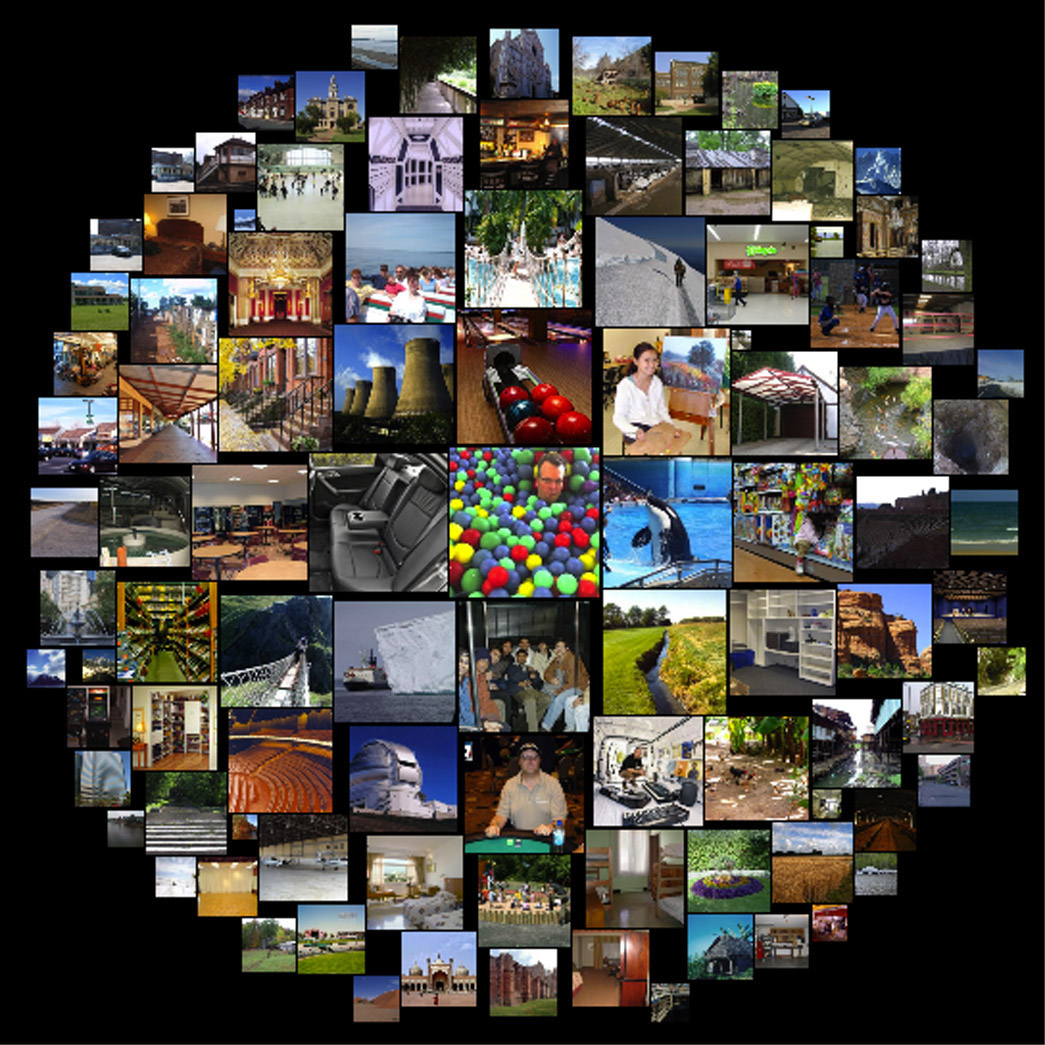
\includegraphics[width=.7\linewidth]{figure/mem_importance.jpg}
    \caption{Sample of the photos used by Isola et al. to develop an algorithm that predicts image memorability. The photos are scaled according to their experimentally measured memorability, with the most memorable photos appearing larger and in the center. Image and caption from \cite{mem_post}.}
    \label{fig:mem_importance}
\end{figure}

To determine the intrinsic features that make an image memorable, Isola et al. first asked 665 individuals from  Amazon Mechanical Turk to participate in a computer memory game. During each level of the game, for up to 30 levels, participants viewed a stream of images and then pressed the space bar whenever they saw one of those images repeated in a subsequent sequence. In total, the image database contained 2222 repeated images and 8220 unrepeated images that included faces, interior-design photos, nature scenes, streetscapes, and others. They found that photographs with people or central objects were memorable, whereas landscapes — that one might expect to be memorable — were among the most forgettable\cite{mem_post}, see Figure \ref{fig:mem_importance}.

Next, Isola et al. assigned a `memorability score' to each image, which was defined as the percent of correct detections by participants in the study. Then they investigated the features of the more memorable images, including color, object statistics (e.g., number of objects or amount of space occupied by objects in the image), object semantics (e.g., what type of object appeared in an image, such as an animal or car), and scene semantics (e.g., the place the image represented, such as a kitchen or landscape). 

Finally they developed an image-ranking algorithm to automatically predict the memorability of images. To do this, Isola et al. trained a support vector regressor — $\epsilon$-SVR implemented on LIBSVM\cite{libsvm} — to map from features to memorability scores using only features algorithmically extracted from the images. The algorithm learned from the memorability scores calculated from the memory game. They used half of the images in the database to train the algorithm and tested its performance with the remaining half. The algorithm correctly identified images with people as most memorable, indoor scenes and large objects as slightly less memorable, and outdoor landscapes as the least memorable.
\section{Predicting Memorability with Statistical Features}
In this section, we are going to discuss the problem of predicting the memorability score using statistical features of images. The images in the dataset were labeled according to the objects included in each of them. For that, Isola et al. have used a tool called LabelMe~\cite{labelme}. Once the images were labeled, we had not only information of what objects were present in the image but also how much area they occupied and their quantity. In total, 9 different features were used to train an $\epsilon$-SVR that predicted the memorability score. The reproduced results along with the results reported in \cite{Isola2011} can be seen in Table \ref{tab:statistical_features}.

\begingroup
\setlength{\tabcolsep}{5pt}
\renewcommand{\arraystretch}{1.5}
\begin{table*}[tb]
\centering
\begin{tabular}{|l||l|l|l|l|l|l|}
\hline
                                                          &            & \textbf{Top 20} & \textbf{Top 100} & \textbf{Bottom 100} & \textbf{Bottom 20} & $\bm{\rho}$ \\ \hline \hline
\multirow{2}{*}{\textbf{Object Counts}}                   & paper      & 0.68            & 0.68             & 0.67                & 0.67               & 0.05       \\ \cline{2-7} 
                                                          & reproduced & 0.68            & 0.68             & 0.68                & 0.68               & 0.03       \\ \hline \hline
\multirow{2}{*}{\textbf{Object Areas}}                    & paper      & 0.67            & 0.68             & 0.64                & 0.63               & 0.05       \\ \cline{2-7} 
                                                          & reproduced & 0.67            & 0.68             & 0.64                & 0.63               & 0.05       \\ \hline \hline
\multirow{2}{*}{\textbf{Multiscale Object Areas}}              & paper      & 0.73            & 0.73             & 0.64                & 0.65               & 0.20       \\ \cline{2-7} 
                                                          & reproduced & 0.73            & 0.73             & 0.64                & 0.65               & 0.19       \\ \hline \hline
\multirow{2}{*}{\textbf{Object Presence}}                 & paper      & 0.84            & 0.79             & 0.57                & 0.55               & 0.43       \\ \cline{2-7} 
                                                          & reproduced & 0.83            & 0.80             & 0.57                & 0.54               & 0.43       \\ \hline \hline
\multirow{2}{*}{\textbf{Labeled Object Counts}}           & paper      & 0.82            & 0.79             & 0.57                & 0.54               & 0.44       \\ \cline{2-7} 
                                                          & reproduced & 0.82            & 0.79             & 0.57                & 0.55               & 0.44       \\ \hline \hline
\multirow{2}{*}{\textbf{Labeled Object Areas}}            & paper      & 0.84            & 0.82             & 0.56                & 0.52               & 0.47       \\ \cline{2-7} 
                                                          & reproduced & 0.84            & 0.82             & 0.57                & 0.53               & 0.48       \\ \hline \hline
\multirow{2}{*}{\textbf{Labeled Multiscale Object Areas}} & paper      & 0.84            & 0.82             & 0.56                & 0.52               & 0.48       \\ \cline{2-7} 
                                                          & reproduced & 0.84            & 0.82             & 0.56                & 0.53               & 0.48       \\ \hline \hline
\multirow{2}{*}{\textbf{Scene Category}}                  & paper      & 0.81            & 0.78             & 0.57                & 0.55               & 0.37       \\ \cline{2-7} 
                                                          & reproduced & 0.81            & 0.77             & 0.58                & 0.56               & 0.36       \\ \hline \hline
\multirow{2}{*}{\textbf{Object and Scenes}}               & paper      & 0.85            & 0.82             & 0.55                & 0.53               & 0.50       \\ \cline{2-7} 
                                                          & reproduced & 0.85            & 0.82             & 0.55                & 0.52               & 0.50       \\ \hline \hline
\multirow{1}{*}{\textbf{Other Humans}}               & paper      & 0.86            & 0.84             & 0.47                & 0.40               & 0.75                 \\ \hline                                            
\end{tabular}
\caption{Results for predicting memorability with statistical features.}
\label{tab:statistical_features}
\end{table*}
\endgroup

\begin{figure*}[htb]
    \centering
    \begin{tabular}{c c c c}
    \rotatebox{90}{Empirical} & 
    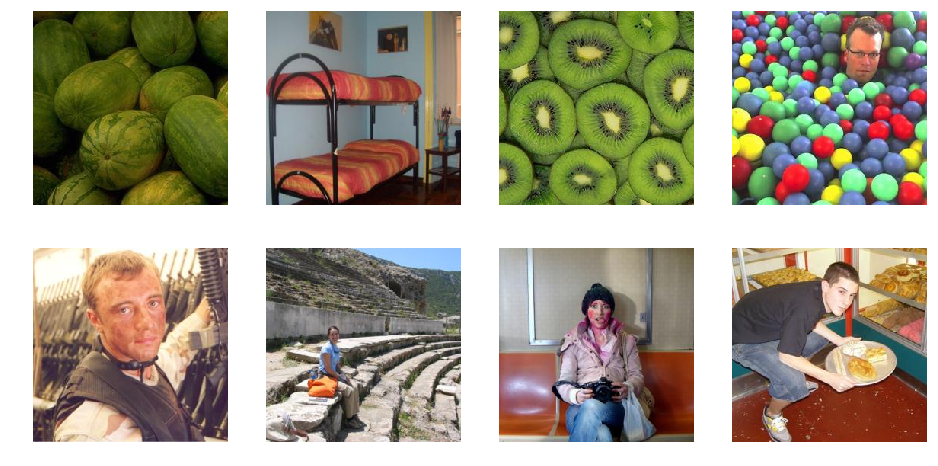
\includegraphics[width=0.3\linewidth]{./figure/empirical_top.png} &
    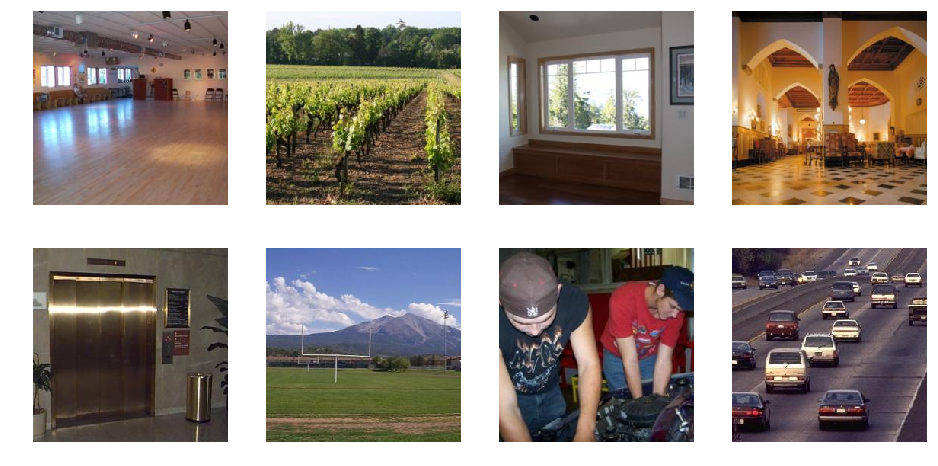
\includegraphics[width=0.3\linewidth]{./figure/empirical_avg.png} &
    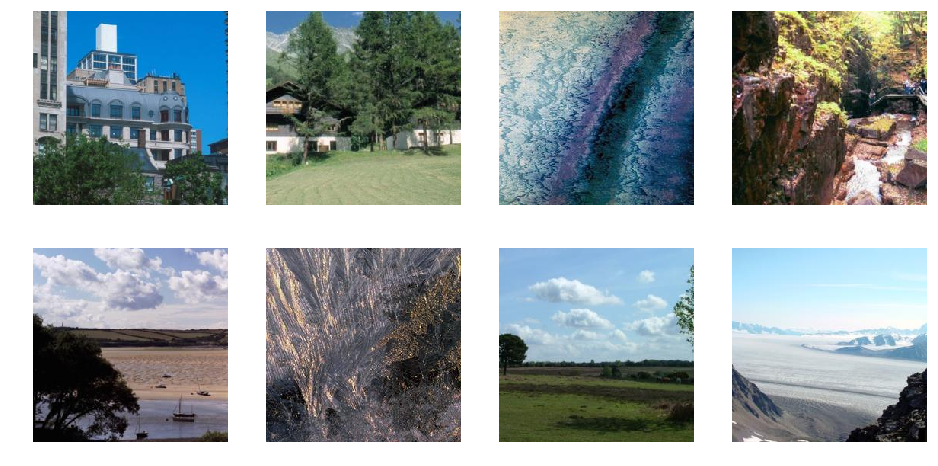
\includegraphics[width=0.3\linewidth]{./figure/empirical_bottom.png}\\
    \rotatebox{90}{Predicted} &
    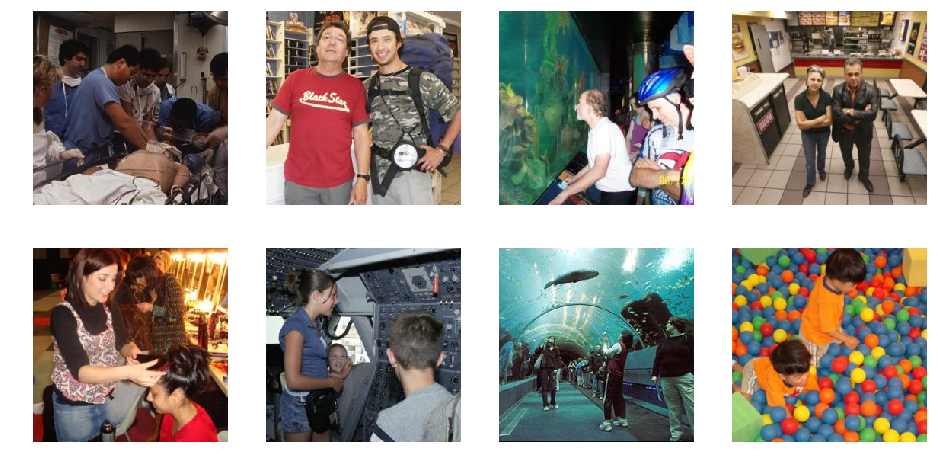
\includegraphics[width=0.3\linewidth]{./figure/predicted_top.png} &
    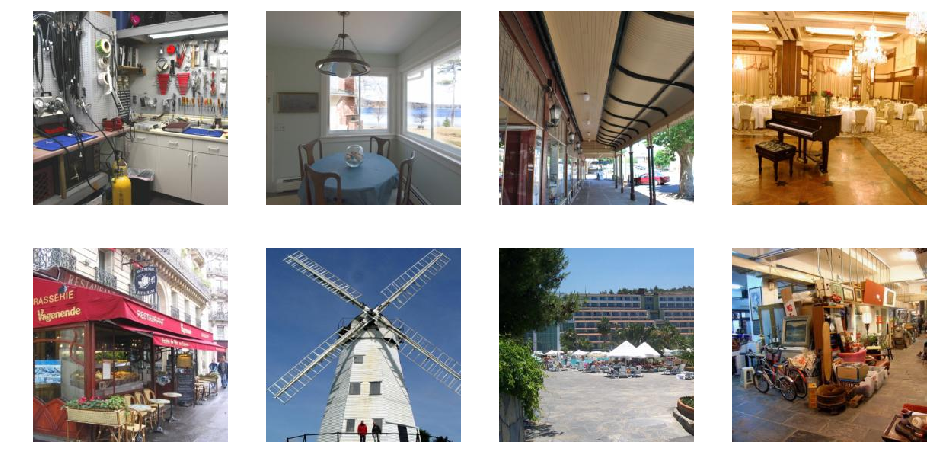
\includegraphics[width=0.3\linewidth]{./figure/predicted_avg.png} &
    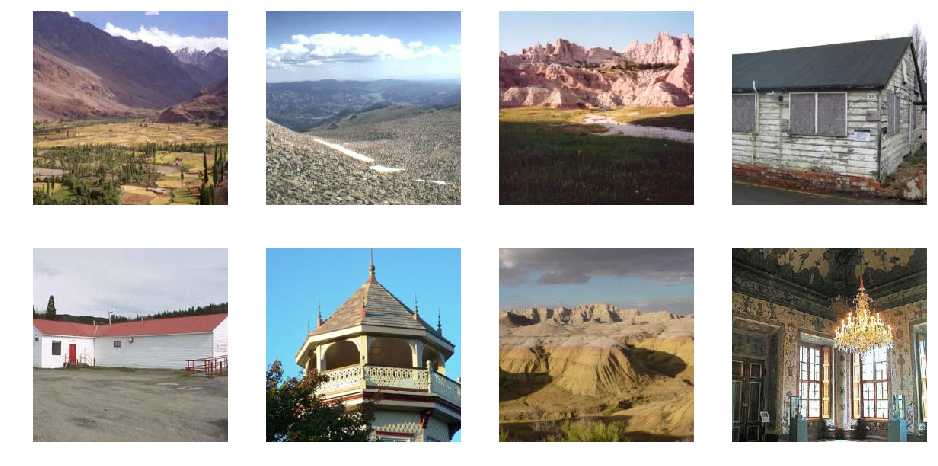
\includegraphics[width=0.3\linewidth]{./figure/predicted_bottom.png}\\
    & a.~Most memorable. & b.~Average memorable. & c.~Least memorable.\\
    \end{tabular}
    \caption{Comparison between empirical and predicted memorability.}
    \label{fig:samples}
\end{figure*}

\subsection{Features}
Although rich information related to the objects in each image was collected, Isola et al. have decided to first explore very basic features consisting solely of object statistics. For every image, the following statistics were gathered: number of objects in the image per class, number of pixels covered by objects of each class in the entire image and number of pixels covered by objects per quadrant in the image. Those were marginalized across object class to generate histograms of ``Object Counts'' and ``Object Areas''. The ``Multiscale Object Areas'' features concatenated pixel coverage on the entire image with pixel coverage per quadrant. These 3 features excluded any semantical information as we did not know anymore what object was or was not included in the image. We only knew their quantities or areas. On the other hand, all the following features considered semantics in the image. The ``Object Presence'' was a binary feature vector stating if the a certain object was or was not part of the image. The ``Labeled Object Counts'' and ``Labeled Object Areas'' contained the count and areas of each class of object respectively. The ``Labeled Multiscale Object Areas'' concatenated the area for each class of object on the entire image with the area per quadrant. A total of 1360 classes of objects were considered in this study. The ``Scene Category'' feature was a binary vector stating which of the 674 scenes the image depicted. The ``Object and Scenes'' was a concatenation of the ``Labeled Multiscale Object Areas'' and the ``Scene Category'' features.

\subsection{Machine Learning: Protocol and Model}
When collecting data from the memorability game, the authors decided to separate 2 different groups of users. The last row in Table \ref{tab:statistical_features} compares the memorability scores measured between the first and second group of users. Data from the first group was used to train the regressor while data from the second was used to test. We are going to call the memorability scores measured from the second group as ``empirical memorability scores''. In general lines, the protocol followed was:
\begin{enumerate}
\item 25 trials: each trial containing 1111 randomly selected images from scores of group 1 and 1111 randomly selected images from scores of group 2.
\item For each trial, perform a grid search to find the optimal hyper parameters cost and $\epsilon$ for SVR.
\item For each combination of hyper parameters, train SVR and predict memorability scores on test dataset on 4 different trials.
\item For each grid search trial, calculate Pearson's product-moment correlation coefficient between the predicted and empirical memorability scores.
\item Average Pearson's product-moment correlation coefficient from the 4 grid search trials.
\item Select the best hyper parameters based on the highest average correlation coefficient.
\item Back to one of the 25 trials, train SVR and predict memorability scores on test dataset with the selected hyper parameters.
\item Average Pearson's product-moment correlation coefficient of the 25 trials. That will be $\rho$ reported in Table \ref{tab:statistical_features}.
\end{enumerate}

In \cite{Isola2011}, the regression model used to predict the memorability score was a $\epsilon$-SVR. They used the ``histogram intersection'' as a kernel. For hyper parameter tuning, a grid search on 49 static combinations of cost and $\epsilon$ was performed.

\subsection{Results}
As one of our objectives in this final project was to reproduce the results from \cite{Isola2011}, we compare our numbers with the ones reported by Isola et al. Table \ref{tab:statistical_features} contains both information. The largest difference found was in the measure $\rho$ for ``Object Counts''. The majority of the results matched exactly with the original paper. None of the results had a difference greater than 2\%.

In Figure \ref{fig:samples}, we analyzed our results from a qualitative perspective. We pulled some 8 samples of images from 3 tiers of memorability: most memorable, average memorable and least memorable. To do that, we simply ordered all images by predicted and empirical memorability scores and then extracted the top 8, mid 8, and bottom 8 images. It is easy to note some resemblance between the images in the ``Empirical'' and ``Predicted'' row. As most memorable, there is a higher concentration of images with people. For least memorable, we can see buildings and landscapes.


\section{Predicting Memorability with Global Features}
As Table~\ref{tab:statistical_features} shows, using semantic information it is possible to obtain good results for predicting memorability. But depending on this kind of information can be somewhat limiting. So, the question now is: can we still predict memorability without using previously labelled data and get good results? To try and answer this question, we turn our attention to global features, which can be computed using no additional information besides the image.

As a first step, we used the features as computed by Isola et al. They used the following feature descriptors: GIST~\cite{gist}, SIFT~\cite{sift}, HOG2x2~\cite{hog}, and SSIM~\cite{ssim}. Additionally, they used pixel histograms. In the case of GIST, an RBF kernel was used, and for the other features, histogram intersection kernels. Also, they experimented with the combination of all these features with a kernel product.

\begingroup
\setlength{\tabcolsep}{5pt}
\renewcommand{\arraystretch}{1.5}
\begin{table*}[ht]
    \centering
    \begin{tabular}{|l||l|c|c|c|c|c|} \hline
         & & \textbf{Top 20} & \textbf{Top 100} & \textbf{Bottom 100} & \textbf{Bottom 20} & $\bm{\rho}$\\ \hline \hline
        \multirow{2}{*}{\textbf{Pixels Histograms}} & Paper & 0.74 & 0.72 & 0.61 & 0.59 & 0.22\\ \cline{2-7}
         & Reproduced & 0.74 & 0.73 & 0.62 & 0.61 & 0.22\\ \hline \hline
        \multirow{2}{*}{\textbf{GIST}} & Paper & 0.82 & 0.78 & 0.58 & 0.57 & 0.38\\ \cline{2-7}
         & Reproduced & 0.82 & 0.79 & 0.58 & 0.57 & 0.38\\ \hline \hline
        \multirow{2}{*}{\textbf{SIFT}} & Paper & 0.83 & 0.79 & 0.57 & 0.56 & 0.41\\ \cline{2-7}
         & Reproduced & 0.83 & 0.80 & 0.57 & 0.55 & 0.42\\ \hline \hline
        \multirow{2}{*}{\textbf{HOG2x2}} & Paper & 0.83 & 0.80 & 0.57 & 0.55 & 0.43\\ \cline{2-7}
         & Reproduced & 0.83 & 0.80 & 0.58 & 0.54 & 0.44\\ \hline \hline
        \multirow{2}{*}{\textbf{SSIM}} & Paper & 0.83 & 0.79 & 0.58 & 0.56 & 0.43\\ \cline{2-7}
         & Reproduced & 0.84 & 0.80 & 0.58 & 0.55 & 0.43\\ \hline \hline
        \multirow{2}{*}{\textbf{All Global Features}} & Paper & 0.83 & 0.80 & 0.56 & 0.54 & 0.46\\ \cline{2-7}
         & Reproduced & 0.83 & 0.80 & 0.56 & 0.53 & 0.46\\ \hline
    \end{tabular}
    \caption{Results for predicting memorability with global features.}
    \label{tab:global_features}
\end{table*}
\endgroup

The results were evaluated in the same manner as we evaluated the statistical features, as is presented in Table~\ref{tab:global_features}. We can see that our results are very similar to the ones from the original paper, differing at most 2\%.

Next, we proceeded to implement our version of the computation of the feature descriptors, based on the usage of the original paper. We implemented our version of pixel histograms, GIST, SIFT, SURF~\cite{surf}, ORB~\cite{orb}, and BRISK~\cite{brisk}. Since pixel histograms are quite simple, we could implement the exact same algorithm as used by Isola et al., yielding the same results as when we used the features computed by them, as can be seen in Table~\ref{tab:our_features}.

\begingroup
\setlength{\tabcolsep}{5pt}
\renewcommand{\arraystretch}{1.5}
\begin{table*}[ht]
    \centering
    \begin{tabular}{|l||l|c|c|c|c|c|} \hline
         & & \textbf{Top 20} & \textbf{Top 100} & \textbf{Bottom 100} & \textbf{Bottom 20} & $\bm{\rho}$\\ \hline \hline
        \multirow{2}{*}{\textbf{Pixels Histograms}} & Paper & 0.74 & 0.72 & 0.61 & 0.59 & 0.22\\ \cline{2-7}
         & Reproduced & 0.74 & 0.73 & 0.62 & 0.61 & 0.22\\ \hline \hline
        \multirow{2}{*}{\textbf{GIST}} & Paper & 0.82 & 0.78 & 0.58 & 0.57 & 0.38\\ \cline{2-7}
         & Reproduced & 0.79 & 0.77 & 0.59 & 0.55 & 0.36\\ \hline \hline
        \multirow{2}{*}{\textbf{SIFT}} & Paper & 0.83 & 0.79 & 0.57 & 0.56 & 0.41\\ \cline{2-7}
         & Reproduced & 0.82 & 0.80 & 0.58 & 0.56 & 0.42\\ \hline \hline
        \multirow{2}{*}{\textbf{SURF}} & Paper & - & - & - & - & -\\ \cline{2-7}
         & Reproduced & 0.77 & 0.76 & 0.59 & 0.56 & 0.35\\ \hline \hline
        \multirow{2}{*}{\textbf{ORB}} & Paper & - & - & - & - & -\\ \cline{2-7}
         & Reproduced & 0.81 & 0.78 & 0.59 & 0.57 & 0.38\\ \hline \hline
        \multirow{2}{*}{\textbf{BRISK}} & Paper & - & - & - & - & -\\ \cline{2-7}
         & Reproduced & 0.79 & 0.76 & 0.60 & 0.57 & 0.34\\ \hline \hline
        \multirow{2}{*}{\textbf{All From Paper}} & Paper & 0.83 & 0.80 & 0.56 & 0.54 & 0.46\\ \cline{2-7}
         & Reproduced & 0.80 & 0.77 & 0.59 & 0.55 & 0.38\\ \hline \hline
        \multirow{2}{*}{\textbf{All Global Features}} & Paper & - & - & - & - & -\\ \cline{2-7}
         & Reproduced & 0.81 & 0.77 & 0.58 & 0.55 & 0.38\\ \hline \hline
        \multirow{2}{*}{\textbf{Best Result}} & Paper & 0.83 & 0.80 & 0.56 & 0.54 & 0.46\\ \cline{2-7}
         & Reproduced & 0.83 & 0.80 & 0.57 & 0.54 & 0.44\\ \hline
    \end{tabular}
    \caption{Results for predicting memorability with computed global features.}
    \label{tab:our_features}
\end{table*}
\endgroup

For the GIST feature descriptor, we used INRIA-LEAR's C implementation~\cite{lear_gist}, with a wrapper for Python provided by Yuichiro Tsuchiya~\cite{tuttieee}. For the SIFT, we used the version provided by OpenCV to implement the dense version, using spatial pyramid histogram~\cite{sift}. As for the dense HOG2x2 used in the paper, we could not find a proper implementation for Python, and could not produce a competitive version based on the HOG implementation found in OpenCV. For this reason, we did not compute HOG descriptors. This was also the case with SSIM.

On the other hand, we could try other feature descriptors, such as SURF, ORB, and BRISK, using the provided implementation from OpenCV and spatial pyramid histograms, like with SIFT. These new descriptors were evaluated using histogram intersection kernels. The results are shown in Table~\ref{tab:our_features} as well.

In Table~\ref{tab:global_features}, the last entry is ``All Global Features'', which means pixels histograms, GIST, SIFT, HOG2x2, and SSIM combined with a kernel product. Since we could not implement all these feature descriptors, we cannot compute this exact same entry. Instead, we computed three entries (the last three entries in Table~\ref{tab:our_features}): ``All From Paper'', ``All Global Features'', and ``Best Result''. The first one represents all descriptors from the original paper that we could implement, namely pixels histograms, GIST, and SIFT, combined. The second one represents all global features computed by us, namely pixels histograms, GIST, SIFT, SURF, ORB, and BRISK, combined. And the ``Best Result'' entry represents the kernel product combination of SIFT, SURF, ORB, and BRISK. In the table, we compare our best result using global features with the best result obtained by Isola et al. in the original paper, using global features as well, even if the features are not the same. To obtain our best result, we tried many combinations (but not every possible combination), such as ``pixels histograms, SIFT, SURF, ORB, and BRISK'', and ``SURF, and ORB'', besides the other already mentioned combinations. In this manner, we could obtain a best result quite similar to the one in the paper, despite the differences in feature descriptors.

Using our version of the global features, we extracted 12 samples of images according to their predicted memorability, as shown in Figure~\ref{fig:images_features}. In the left, we have 4 sample images that were predicted most memorable; in the middle, 4 sample images that were predicted with average memorability; and in the right, 4 sample images that were predicted least memorable. To obtain these images, a process analogous to the one used to build Figure~\ref{fig:samples} was used here. Using global features, we have a similar tendency as the previous methods: images with people being more memorable, and images of landscapes being less memorable.

\begin{figure*}[ht]
    \centering
    \begin{tabular}{c c c c c}
        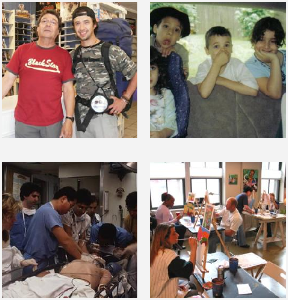
\includegraphics[width=0.3\linewidth]{./figure/features_top.png} & &
        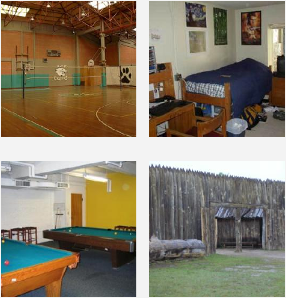
\includegraphics[width=0.3\linewidth]{./figure/features_average.png} & &
        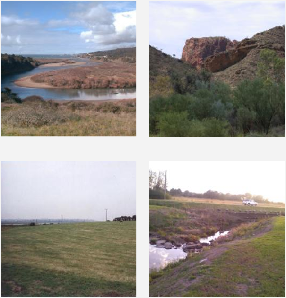
\includegraphics[width=0.3\linewidth]{./figure/features_bottom.png} \\
        a.~Predicted memorable. & & b.~Predicted average. & & c.~Predicted forgettable.
    \end{tabular}
    \caption{Example of images according to the predicted memorability using global features.}
    \label{fig:images_features}
\end{figure*}


\section{What content makes an image memorable?}
Among the many reasons why an image might be remembered by a viewer, Isola et al. investigate at first the following factors: color, simple image features, object statistics, object semantics, and scene semantics.

\textbf{Color and simple image features}. Isola et al. looked at the correlation between memorability and basic pixel statistics and discovered that mean hue was weakly predictive of memory: as mean hue transitions from red to green to blue to purple, memorability tends to go down. Also, mean saturation and value, on the other hand, as well as the first three moments of the pixel intensity histogram, exhibited weaker correlations with memorability. 

\begin{figure*}[t]
  \centering
  \begin{tabular}{c c c}
  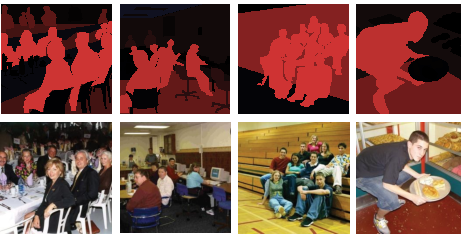
\includegraphics[width=0.33\linewidth]{figure/memorability/mem_top.pdf} &
  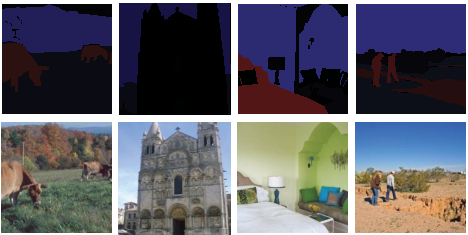
\includegraphics[width=0.33\linewidth]{figure/memorability/mem_middle.pdf} &
  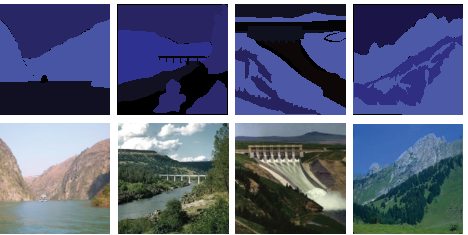
\includegraphics[width=0.33\linewidth]{figure/memorability/mem_botom.pdf}\\
  a.~Predicted as highly memorable. & b.~Predicted as typical memorable & c.~Predicted unmemorable.\\
  \end{tabular}
%   \vspace{-4pt}
  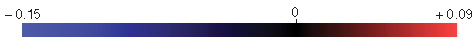
\includegraphics[width=.5\linewidth]{figure/memorability/mem_scale.pdf}
  \caption{Memorability maps from Isola et. al. Higher values in the scale (red in the maps) show the importance of a given object to the memorability.}
  \label{fig:mem_map}
\end{figure*}

\textbf{Object statistics}. Each image in the target set was segmented into object regions and each of these segments was given an object class label by a human user (e.g. ``person'', ``mountain'', ``stethoscope''). Isola et al. found that simple object statistics such as log number of objects, log mean pixel coverage over present object classes, and log max pixel coverage over object classes do not correlate strongly with memorability. They have trained a support vector regression $\epsilon$-SVR to map object statistics to memorability scores. For each image, we measured several object statistics: the number of objects in the image per class, and the number of pixels covered by objects of each class in the entire image as well as in each quadrant of the image.

\textbf{Object and scene semantics}. As found in Isola et al., objects without semantics are not effective at predicting memorability. To investigate the role of object semantics, they performed the same regression as the previous paragraph, but this time using the semantics of the image, that is, the labels from the ground-truth semantic segmentation.

Then Isola et al. conclude that content appears to be important in determining whether or not an image will be remembered, thus they decided to investigate the contribution of objects by visualizing object-based ``memory maps'' for each image, that is, how important is a given object in terms of its semantic segmentation and the proportion of memorability of it. These maps shade each object according to how much the object adds to, or subtracts from, the image's predicted memorability.

To quantify a contribution of an object $i$, we use the prediction function $f$, in this case $\epsilon$-SVR, that maps object features to memorability scores and calculate how its prediction $m$ changes when we have zero features associated with the object $i$ from the current image's feature vector $a_i$:

\begin{ceqn}
\begin{align*}
    m_1 &= f(a_1, \dots, a_i, \dots, a_n)\\
    m_2 &= f(a_1, \dots, 0, \dots, a_n)\\
    s_i &= m_1 - m_2
\end{align*}
\end{ceqn}

As in the original paper, we use SVR on Labeled Multiscale Object Areas and we compute which objects are important across all images by computing $s_i$ for the features of object $i$ across all test set images in which it appears with substantial size (covers over 4000 pixels). Isola et. al. sorted the objects by the averaged memorability importance across images, we get the following ordering: people, interiors, foregrounds, and human-scale objects tend to contribute positively to memorability; exteriors, wide-angle vistas, backgrounds, and natural scenes tend to contribute negatively to memorability.

Isola et al. plotted the memory maps in order to give a sense of how objects contribute to the memorability of particular images. In our experiments, the $\epsilon$-SVR used was the one provided by Scikit-Learn, which is different from the original paper, and somehow we were not able to predict good value of memorability, and thus some of the images chosen as test yield a low quantity of objects and we could not use their precomputed semantic segments of the images. In Figures \ref{fig:mem_map}a, \ref{fig:mem_map}b and \ref{fig:mem_map}c we can see the importance of the objects of an image to its memorability. Their analysis of object semantic regressions demonstrates that if a system knows which objects an image contains, it is able to predict memorability close the human consistency.


%\section{Discussion}


\section{Conclusion}
A few conclusions could be drawn from the reproduced paper. Firstly, it is clear that memorability is an intrinsic property of images which can be measured across different user groups with consistency. Moreover, memorability can be predicted with a fair accuracy using computer vision, machine learning, and global features. Lastly, we confirmed that images with people tend to have higher memorability scores than images containing only buildings or landscapes. In other words, the content of the image plays a big role on how memorable it is going to be.

{\small
\bibliographystyle{ieee}
\bibliography{egbib}
}

\end{document}
